\documentclass{article}
\usepackage{tikz}
\usetikzlibrary{shapes.geometric, arrows, positioning, fit, backgrounds, calc}

\begin{document}

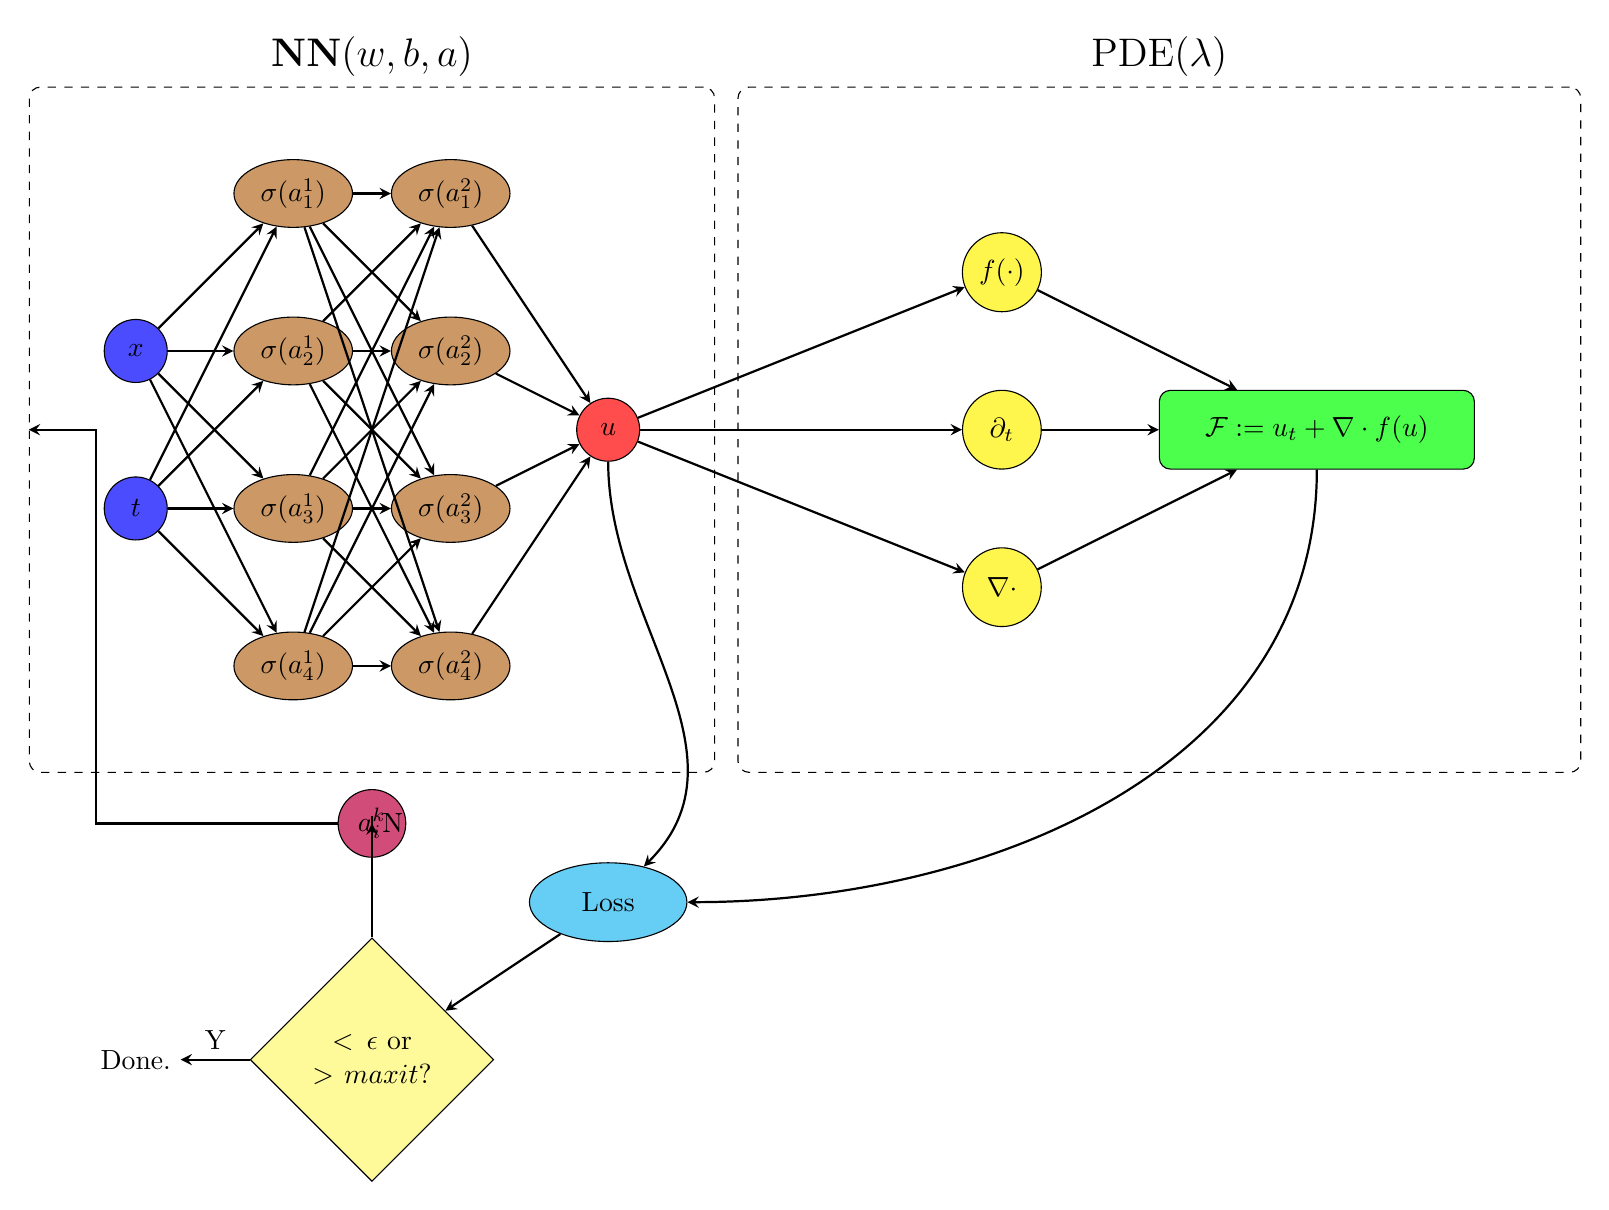
\begin{tikzpicture}[
    % Define node styles
    neuron/.style={ellipse, draw, fill=brown!80, minimum width=1.3cm, minimum height=0.8cm},
    input/.style={circle, draw, fill=blue!70, minimum size=0.8cm},
    output/.style={circle, draw, fill=red!70, minimum size=0.8cm},
    pde/.style={circle, draw, fill=yellow!70, minimum size=1cm},
    operation/.style={rectangle, draw, fill=green!70, rounded corners, minimum width=4cm, minimum height=1cm},
    loss/.style={ellipse, draw, fill=cyan!60, minimum width=2cm, minimum height=1cm},
    decision/.style={diamond, draw, fill=yellow!40, text width=2cm, align=center},
    arrow/.style={thick, ->, >=stealth},
    box/.style={rectangle, draw, dashed, rounded corners, inner sep=10pt}
]

% Neural Network part
\coordinate (nn_top_left) at (-7,4);
\coordinate (nn_bottom_right) at (1,-4);
\node[box, fit={(nn_top_left) (nn_bottom_right)}] (nn) {};
\node[above] at (nn.north) {\Large \textbf{NN}$(w, \boldsymbol{b}, \boldsymbol{a})$};

% Input layer
\node[input] (x) at (-6,1) {$\boldsymbol{x}$};
\node[input] (t) at (-6,-1) {$t$};

% Hidden layers
\node[neuron] (h11) at (-4,3) {$\sigma(a_1^1)$};
\node[neuron] (h12) at (-4,1) {$\sigma(a_2^1)$};
\node[neuron] (h13) at (-4,-1) {$\sigma(a_3^1)$};
\node[neuron] (h14) at (-4,-3) {$\sigma(a_4^1)$};

\node[neuron] (h21) at (-2,3) {$\sigma(a_1^2)$};
\node[neuron] (h22) at (-2,1) {$\sigma(a_2^2)$};
\node[neuron] (h23) at (-2,-1) {$\sigma(a_3^2)$};
\node[neuron] (h24) at (-2,-3) {$\sigma(a_4^2)$};

% Output
\node[output] (u) at (0,0) {$u$};

% Connect input to first hidden layer
\draw[arrow] (x) -- (h11);
\draw[arrow] (x) -- (h12);
\draw[arrow] (x) -- (h13);
\draw[arrow] (x) -- (h14);
\draw[arrow] (t) -- (h11);
\draw[arrow] (t) -- (h12);
\draw[arrow] (t) -- (h13);
\draw[arrow] (t) -- (h14);

% Connect first hidden layer to second hidden layer
\foreach \i in {1,2,3,4}
    \foreach \j in {1,2,3,4}
        \draw[arrow] (h1\i) -- (h2\j);

% Connect second hidden layer to output
\draw[arrow] (h21) -- (u);
\draw[arrow] (h22) -- (u);
\draw[arrow] (h23) -- (u);
\draw[arrow] (h24) -- (u);

% PDE part
\coordinate (pde_top_left) at (2,4);
\coordinate (pde_bottom_right) at (12,-4);
\node[box, fit={(pde_top_left) (pde_bottom_right)}] (pde) {};
\node[above] at (pde.north) {\Large PDE$(\lambda)$};

\node[pde] (f) at (5,2) {$f(\cdot)$};
\node[pde] (dt) at (5,0) {$\partial_t$};
\node[pde] (nabla) at (5,-2) {$\nabla \cdot$};

\node[operation] (residual) at (9,0) {$\mathcal{F}:= u_t + \nabla \cdot f(u)$};

% Connect PDE components
\draw[arrow] (u) -- (f);
\draw[arrow] (u) -- (dt);
\draw[arrow] (u) -- (nabla);
\draw[arrow] (f) -- (residual);
\draw[arrow] (dt) -- (residual);
\draw[arrow] (nabla) -- (residual);

% Loss function and training control
\node[loss] (loss) at (0,-6) {Loss};

% Adaptive parameter node
\node[circle, draw, fill=purple!70, minimum size=0.8cm] (adapt) at (-3,-5) {$a_i^k$};

% Decision diamond
\node[decision] (decision) at (-3,-8) {$< \epsilon$ or\\$> maxit?$};

% Final state
\node (done) at (-6,-8) {Done.};

% Connect other components
\draw[arrow] (u) to[out=-90, in=45] (loss);
\draw[arrow] (residual) to[out=-90, in=0] (loss);
\draw[arrow] (loss) -- (decision);
\draw[arrow] (decision) -- node[above] {Y} (done);
\draw[arrow] (decision) |-node[right] {N} (adapt);

% L-shaped arrow from adapt to nn
\path (adapt) -- ++(-3.5,0) coordinate (aux1);
\path (aux1) -- ++(0,5) coordinate (aux2);
\draw[arrow] (adapt) -- (aux1) -- (aux2) -- (nn.west);

\end{tikzpicture}

\end{document}
